\documentclass{article}
\usepackage{graphicx}
\usepackage{subfigure}

\begin{document}

\title{{\sc dfnWorks} test case tutorial}
\maketitle

This document contains a short, three example, tutorial for {\sc dfnWorks}. The three test cases provided are: test\_4fractures, test\_100fractures, and test\_1000 fractures.  Each of the examples has their own directories, in which is a shell script to execute the program. Also within the directory there are input files for mathematica, pflotran and particle tracking.
The focus of this document is to provide visual confirmation that new users of {\sc dfnWorks} have the code set up correctly, can carry out the following runs and reproduce the following images. 
All images are rendered using Paraview, which can be obtained for free at $http://www.paraview.org/$.\\\\
The examples become more complicated with number of fractures. 
We recommend that you proceed in the order that they are presented here. 
Also, due to the stochastic nature of the DFN, those with newer mathematic, (9 or 10), might not get the exact same DFN, due to possible changes in the mathematica random number generation methodology. 
Variability might also be observed in particle trajectories, for similar reason. 

\noindent {\bf Execution:}

To run one of the test case enter the following type of command (INPUT PARAMETERS WILL CHANGE FOR ACTUAL RUNS):

\begin{itemize}
\item ./runDFN\_environmental\_variables.sh jobname input.m ncpu
\end{itemize}

\noindent The shell scripts takes three command line inputs\\

\noindent input\_1: jobname : a new folder named jobname will be created in the current directory, all files will be produced therein\\
    
\noindent input\_2: input.m : mathematica input file\\

\noindent input\_3: number of cpus (integer) Number of CPUs used for parallel meshing of fractures and in {\sc PFLOTRAN}\\


\noindent This command will create a folder $jobname$ and use the parameters in $input.m$ to generate a fracture network in that folder. Meshing and flow solution will be computed using $ncpu$ processors. 

For example, to run the demo problem test\_4fractures on 4 cpus, the command line input would be:\\\\
 ./runDFN\_environmental\_variables.sh test\_4fractures input\_4fracturetest.m 4\\

This will create a new folder test\_4fractures where all output files will be located. 
Details of what each output file is are in dfnWorks-README.txt.   In the following sections, we provide descriptions of three examples. Each example is in a different folder, to which you must navigate first.

\section{test\_4fractures}

This test case consists of four user defined fractures within a a cubic domain with sides of length one meter. 
To run the demo problem test\_4fractures on 4 cpus, enter the following command line input:\\\\
 ./runDFN\_environmental\_variables.sh test\_4fractures input\_4fracturetest.m 4\\\\
 This will create a new folder, test\_4fractures, where all of the output will be located. 
You can compare your run to the samples provides in the directory test\_results, specifically the output file test.out.
You should also compare your results to the following images. 

\begin{center}
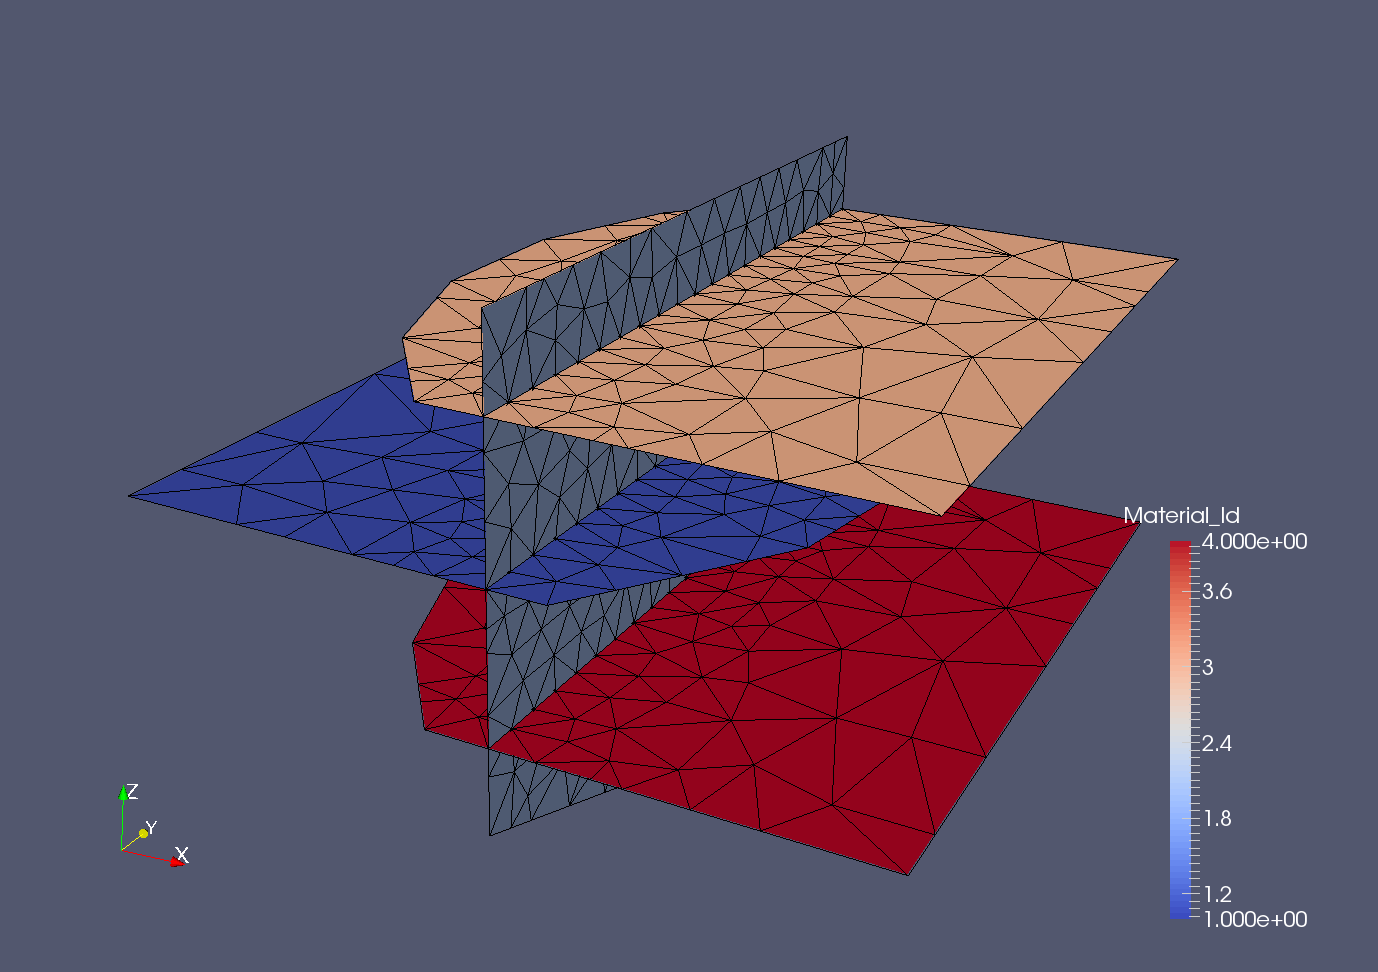
\includegraphics[width=0.75\linewidth]{figs/test_4_fracture_mesh.png}\\
\end{center}
The network of four fractures, each colored by material ID. 
The computational mesh is overlaid on the fractures. 
This image is created by loading the file $full\_mesh.inp$ into paraview. 



\begin{center}
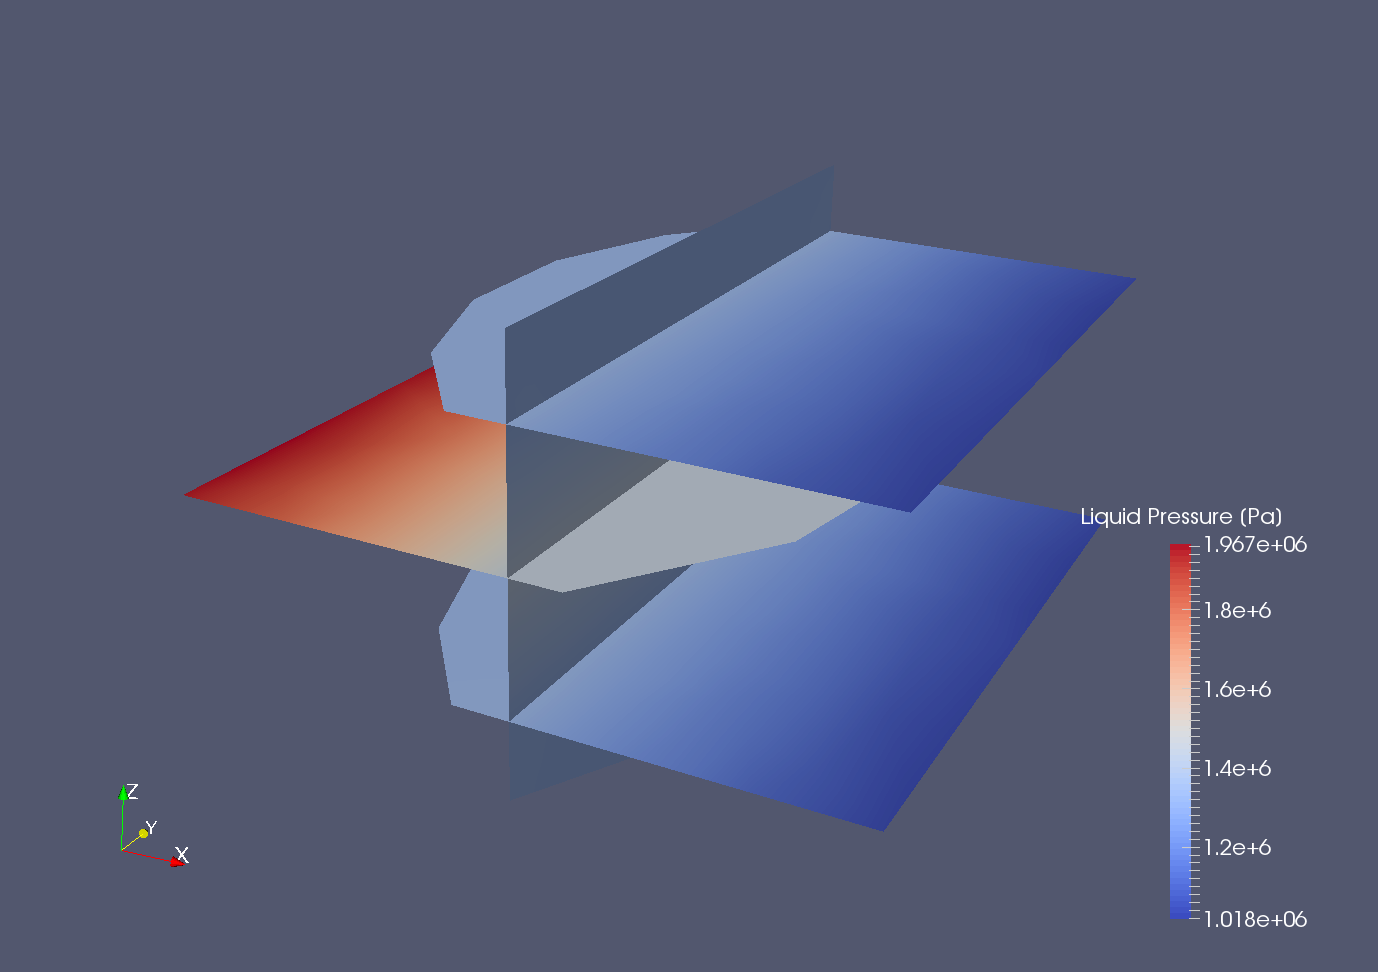
\includegraphics[width=0.75\linewidth]{figs/test_4_fracture_pressure.png}\\
\end{center}
The network of four fractures,  colored by pressure solution.  
High pressure (red) Dirichlet boundary conditions are applied on the edge of the single fracture along the boundary $x = -0.5$, and low pressure (blue)  boundary conditions are applied on the edges of the two fractures at the boundary $x = 0.5$.
This image is created by loading the file $dfn\_explicit-001.xmf$.


%Figure~\ref{fig:test_case4_trajectories} shows particle trajectories on the network of four fractures.   
%Particles are inserted uniformly along the inlet fracture on the left side of the image. 
%They reach the vertical fracture, and either move upwards, downwards, or a single particle continues through on the same fracture, note the arch in eh center of the image.
%Particles exit the domain through the two horizontal fractures on the right side of the image.  
%Trajectories are colored by the current velocity magnitude of the particle's velocity. 
%Trajectories can be visualized by loading the files part\_*.inp. 
% We have used the extract surface and tube filters in paraview for visual clarity. 
\begin{center}
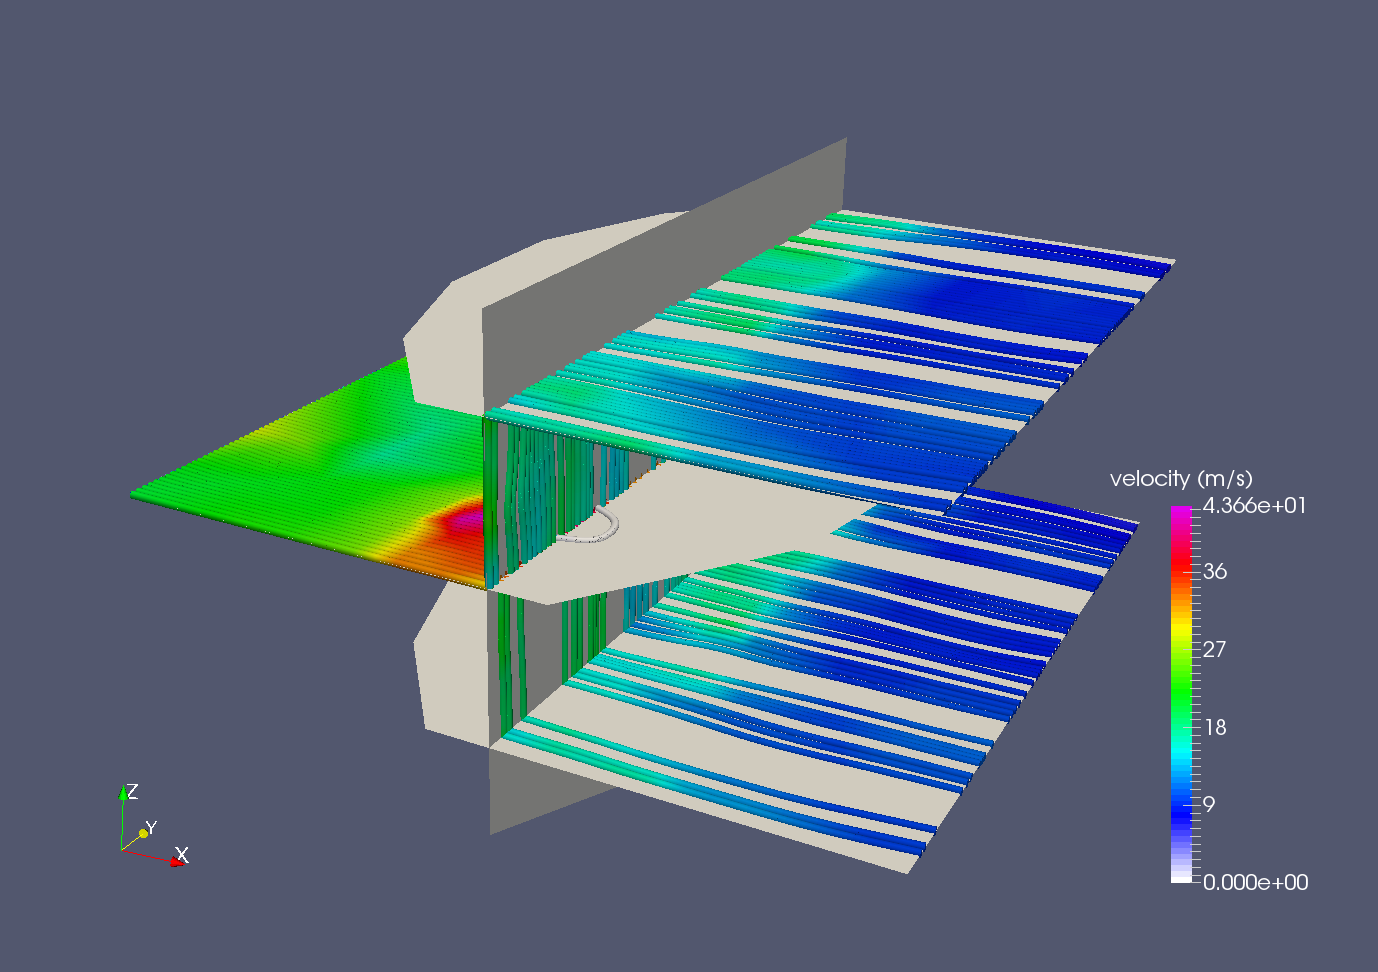
\includegraphics[width=0.75\linewidth]{figs/test_4_fracture_trajectories.png}\\
\end{center}
 Particle trajectories on the network of four fractures.   
Particles are inserted uniformly along the inlet fracture on the left side of the image. 
Particles exit the domain through the two horizontal fractures on the right side of the image.  
Due to the stochastic nature of the particle tracking algorithm, your pathlines might not be exactly the same as in this image. 
Trajectories are colored by the current velocity magnitude of the particle's velocity. 
Trajectories can be visualized by loading the files part\_*.inp. 
 We have used the extract surface and tube filters in paraview for visual clarity. 


\newpage 

\newpage

\section{test\_100fractures}

This test contains 77 rectangular fractures in a cubic domain, box size 10 x 10 x10. 
 Flow goes from bottom to top, and particles are seeded uniformly.    
To run the demo problem test\_100fractures on 8 cpus, enter the following command line input:\\\\
 ./runDFN\_environmental\_variables.sh test\_100fractures test\_input100.m 8\\\\
 This will create a new folder, test\_100fractures, where all of the output will be located. 
 8 CPUS will be used for meshing and the flow solution. 
You can compare your run to the samples provides in the directory test\_results, specifically the output file test.out.
You should also compare your results to the following images. 


\begin{center}
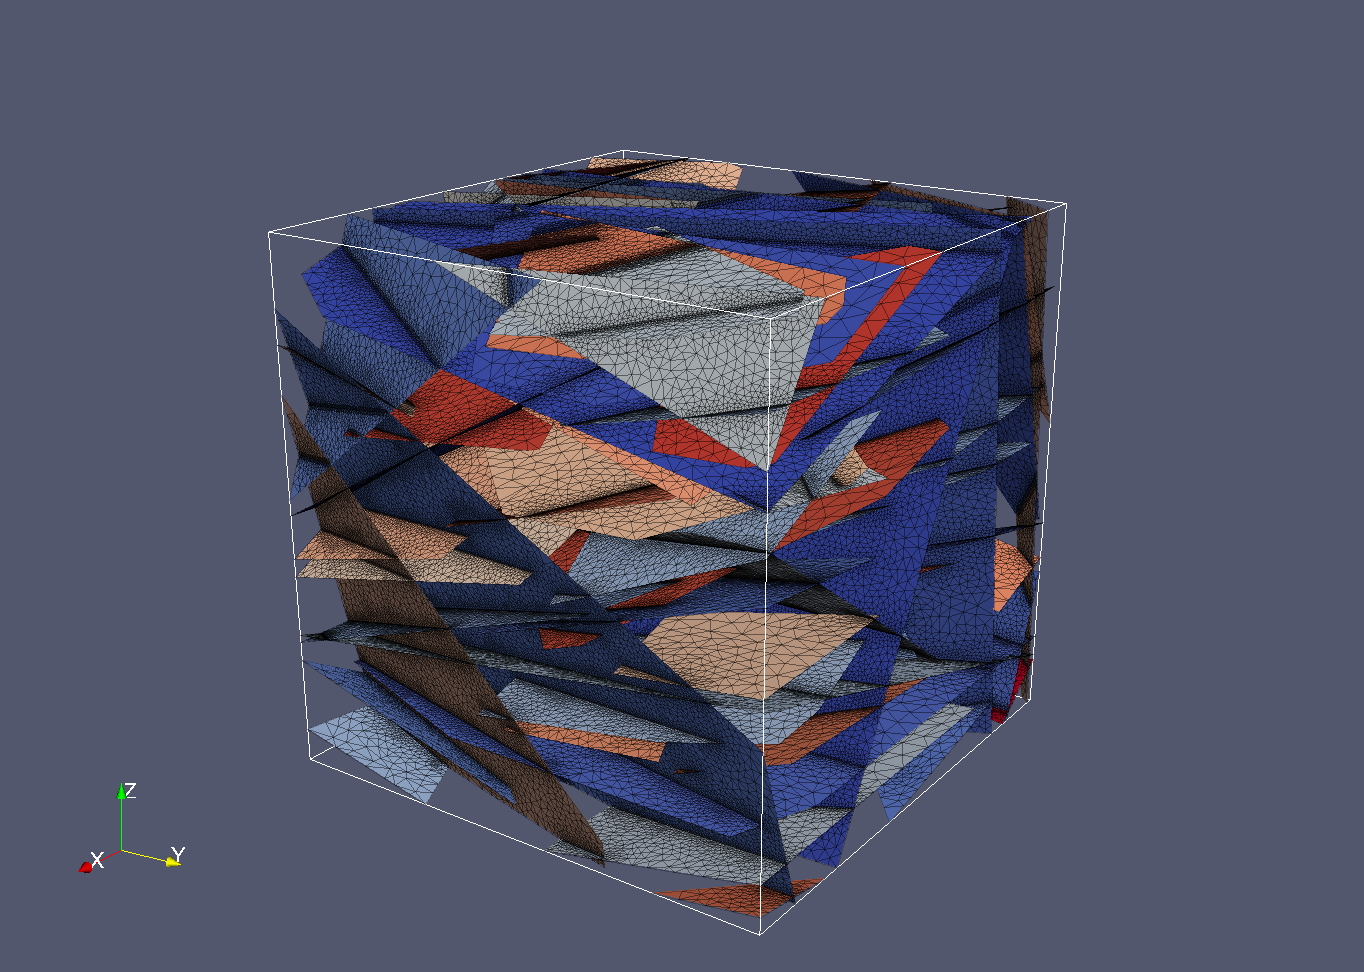
\includegraphics[width=0.75\linewidth]{figs/test_100_fracture_mesh.png}\\
\end{center}
The network of 77 fractures, each colored by material ID. 
The computational mesh is overlaid on the fractures. 
This image is created by loading the file $full\_mesh.inp$


\begin{center}
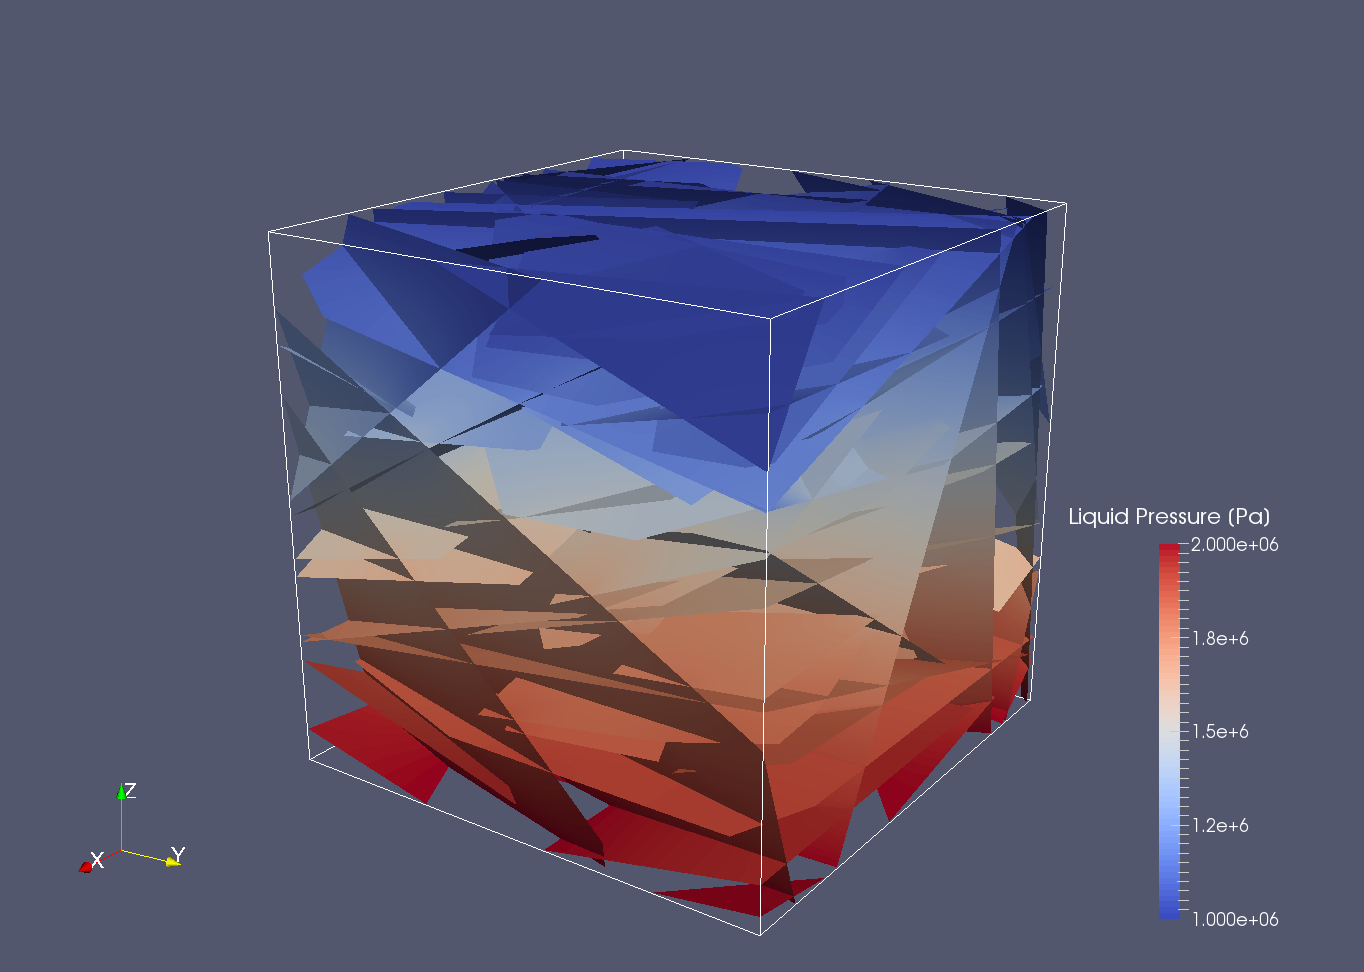
\includegraphics[width=0.75\linewidth]{figs/test_100_fracture_pressure.png}\\
\end{center}
The network of 77 fractures,  colored by pressure solution.  
High pressure (red) Dirichlet boundary conditions are applied on the bottom of the domain, and low pressure (blue)  boundary conditions are applied on the top of the domain. 
This image is created by loading the file $dfn\_explicit-001.xmf$.

\begin{center}
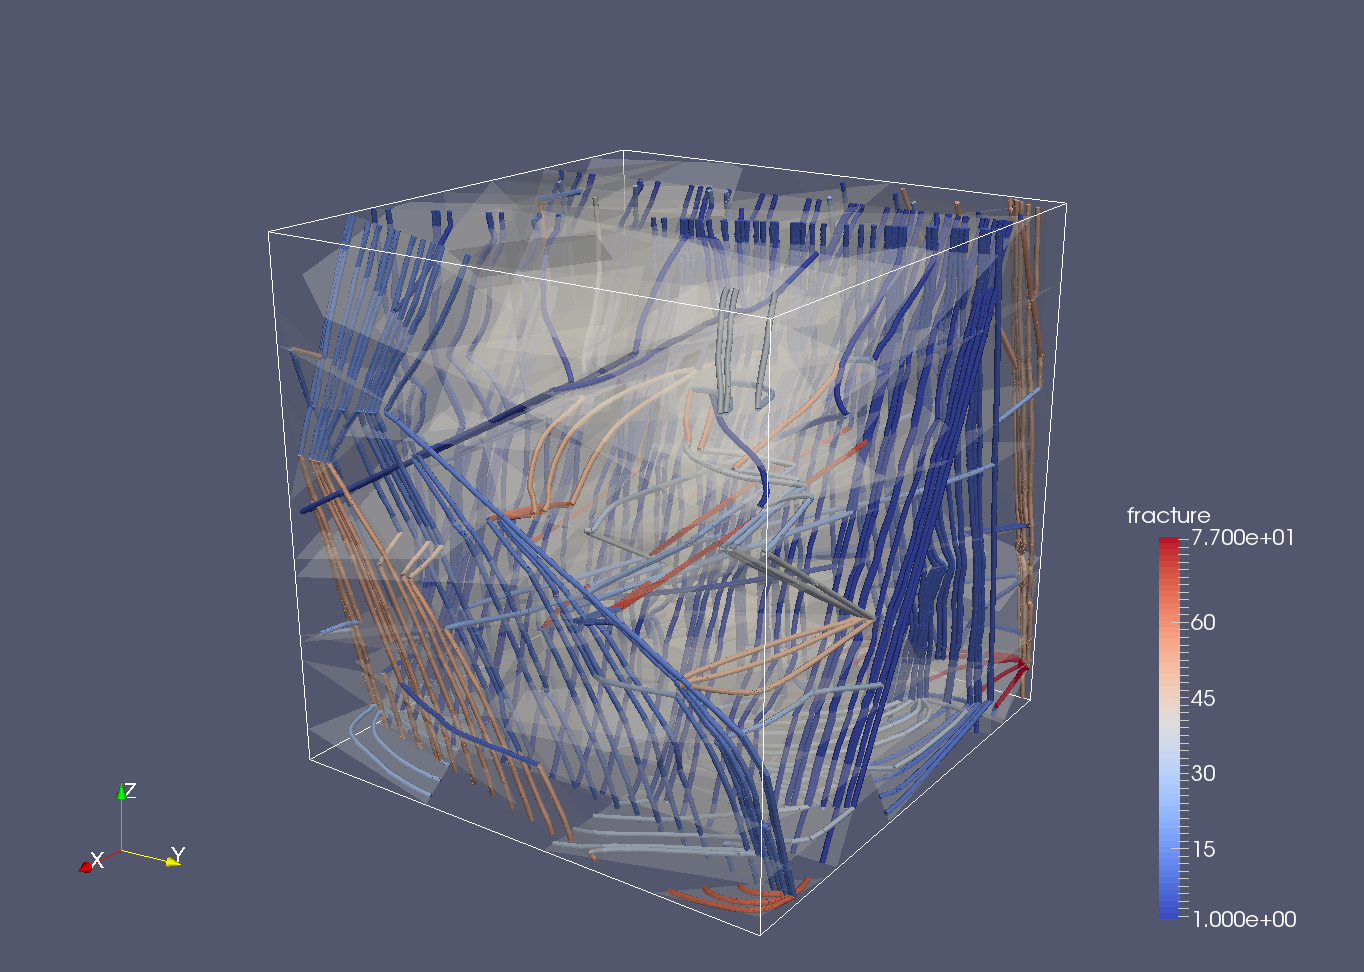
\includegraphics[width=0.75\linewidth]{figs/test_100_fracture_trajectories.png}\\
\end{center}
Particle trajectories in the medium sized network.    
Particles are inserted uniformly along fractures on the bottom of the domain.  
Trajectories are colored by the current fracture network. 
Trajectories can be visualized by loading the files $part\_*.inp$. 
 We have used the extract surface and tube filters in paraview for visual clarity. 
The networks shown with opacity of 0.1 to demonstrate how particles transition between fractures.


\newpage 

\section{test\_1000fractures}

This test case consists This DFN contains 1475 elliptical fractures, and flow goes from front to back. along y axes. Particles are seeded from a point source . In 
To run the demo problem test\_1000fractures on 32 cpus, enter the following command line input:\\\\
 ./runDFN\_environmental\_variables.sh test\_1000fractures test\_input1000.m 32\\\\\
 This will create a new folder, test\_1000fractures, where all of the output will be located. 
You can compare your run to the samples provides in the directory test\_results, specifically the output file test.out.
You should also compare your results to the following images. 


\begin{center}
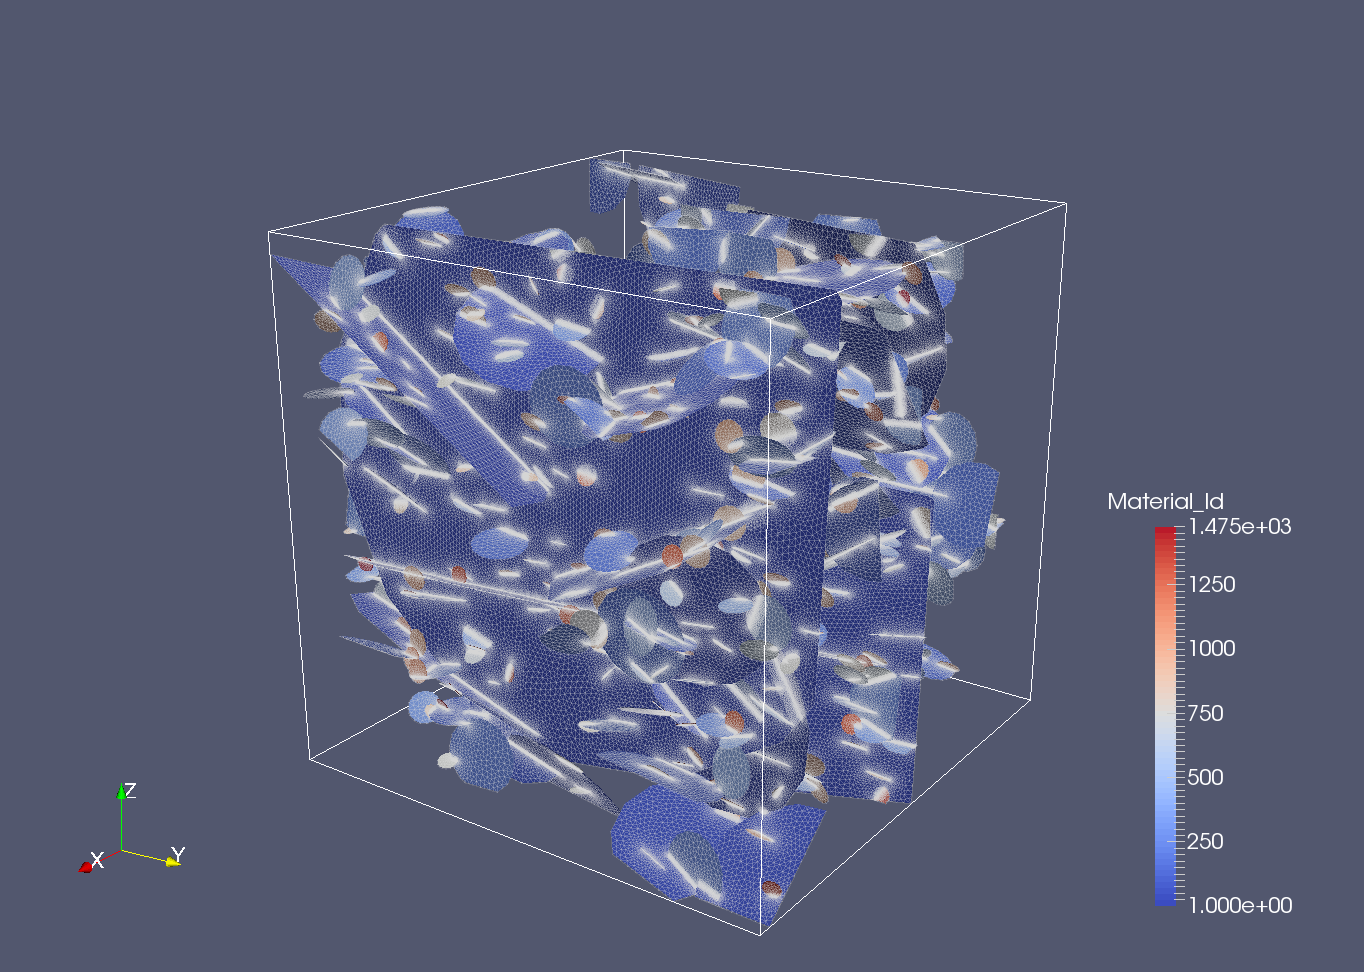
\includegraphics[width=0.75\linewidth]{figs/test_1000_fracture_mesh.png}\\
\end{center}
Network of network of 1475 fractures, each colored by material ID. 
The computational mesh is overlaid on the fractures in white, notice the high resolution near fracture intersections.  
This image is created by loading the file $full\_mesh.inp$

\begin{center}
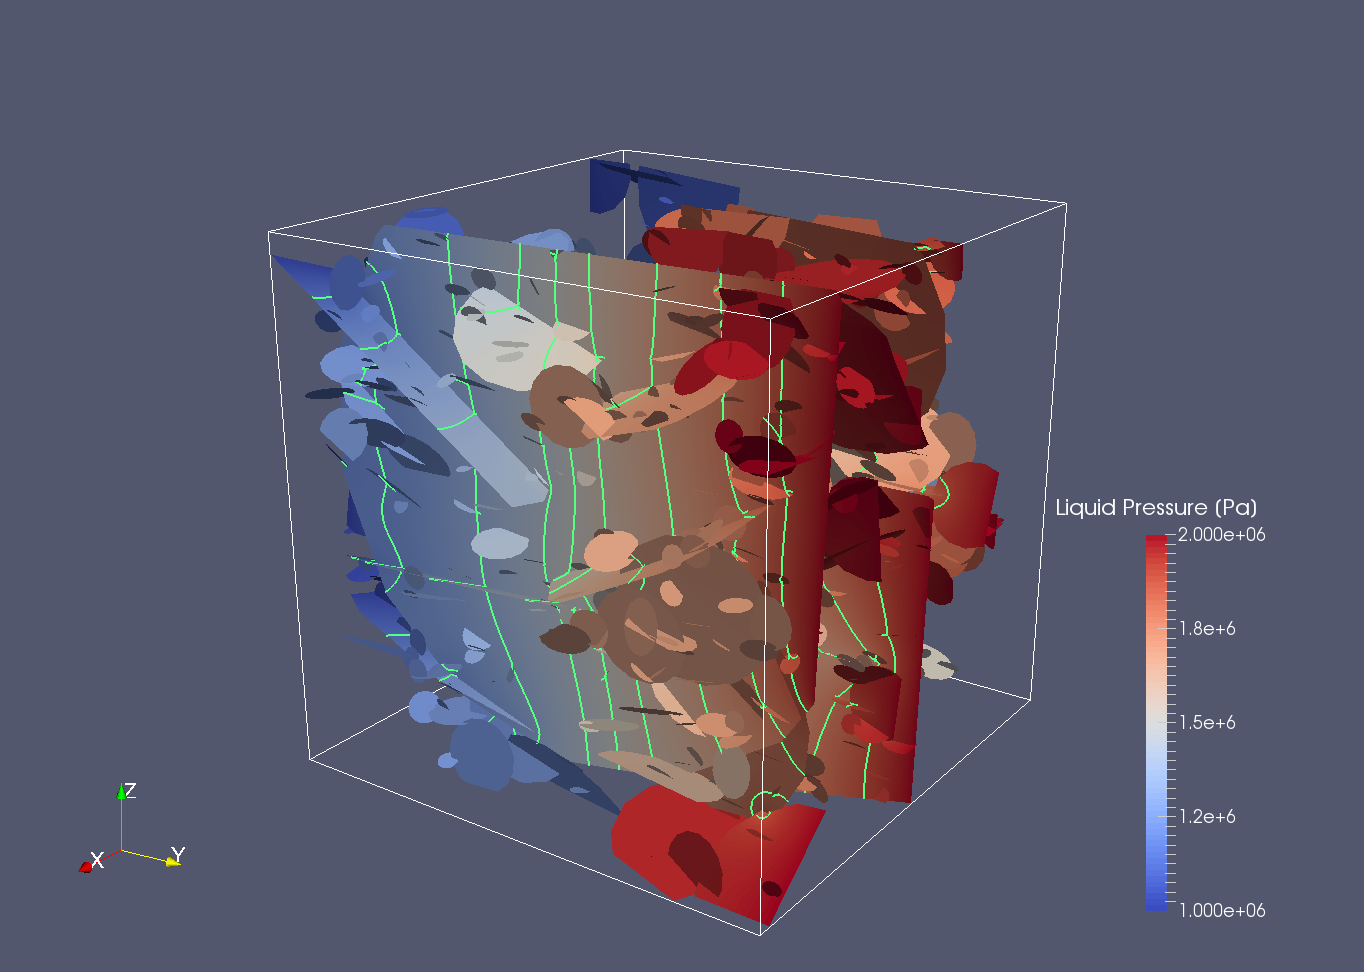
\includegraphics[width=0.75\linewidth]{figs/test_1000_fracture_pressure.png}\\
\end{center}
Network of 1475 fractures,  colored by pressure solution.  
High pressure (red) Dirichlet boundary conditions are applied on the right side of the domain, and low pressure (blue)  boundary conditions are applied on the left side of the domain. 
Pressure contours are shown in green. 
This image is created by loading the file $dfn\_explicit-001.xmf$.



\begin{center}
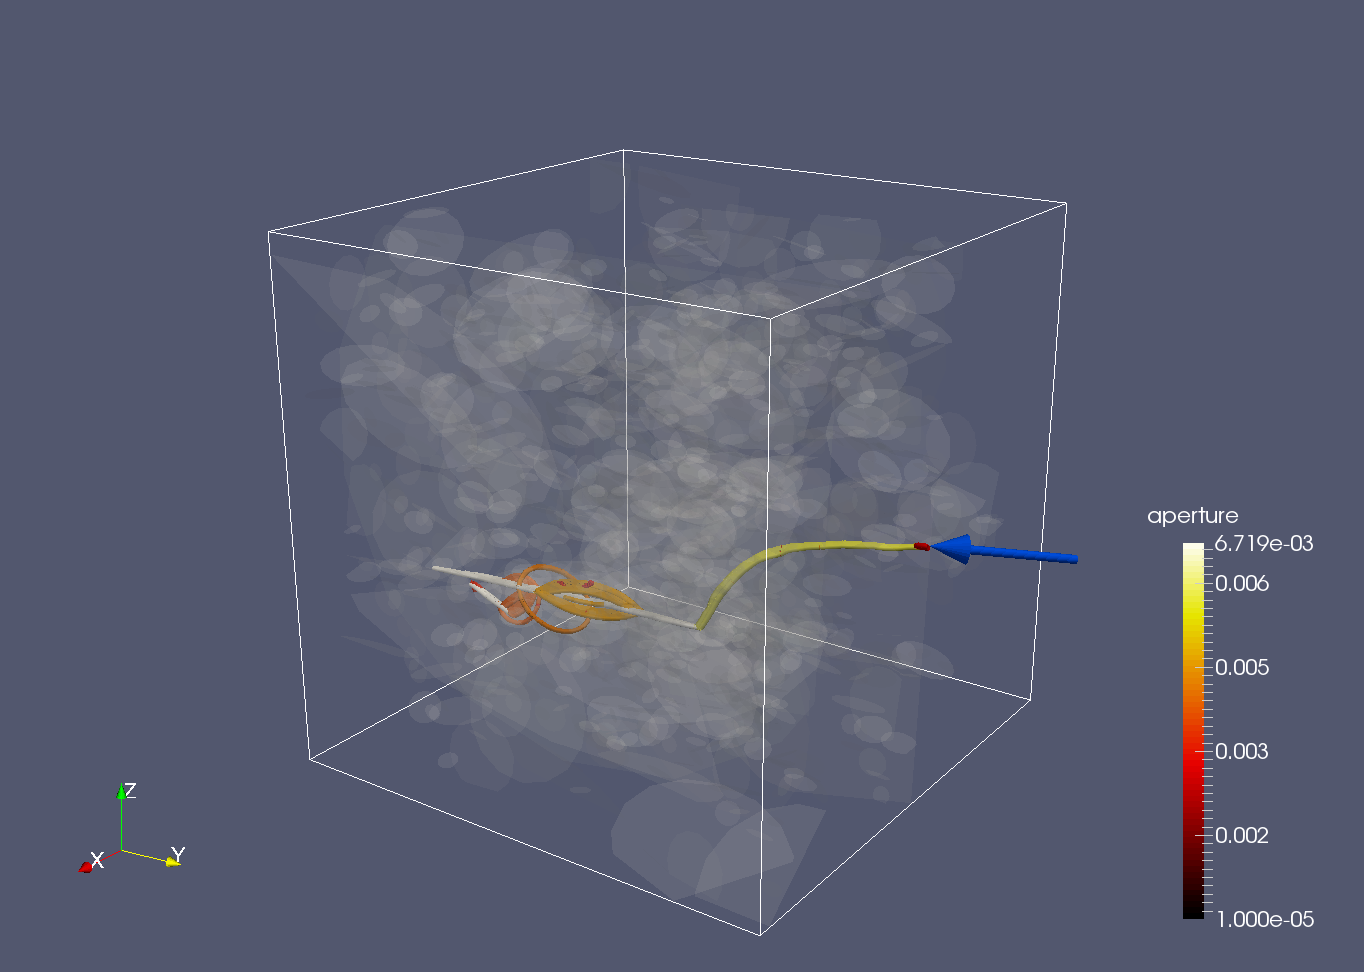
\includegraphics[width=0.75\linewidth]{figs/test_1000_fracture_trajectories.png}\\
\end{center}
Particle trajectories in the large network.    
Particles are inserted uniformly along fractures on the right boundary of the domain.  
Trajectories are colored by the current aperture of the fracture on which they reside. 
The arrow on the right side of the image indicates the initial injection point. 
Trajectories can be visualized by loading the files $part\_*.inp$. 
 We have used the extract surface and tube filters in paraview for visual clarity. 
The networks shown with opacity of 0.1 to demonstrate how particles transition between fractures.




\end{document}
